\subsection{Vorzeitiges Laden von Templates}
\label{pt-tp-main}
Unter dem vorzeitigen Laden von \glspl{Template} versteht man das Zwischenspeichern des \gls{html}-Codes einer Seite vor dem eigentlichen Anzeigen der Seite. Ziel ist es, den ersten Seitenaufruf zu beschleunigen, indem der Inhalt nicht erst über die Netzwerkschnittstelle geladen werden muss. 
\\\\
Das Prinzip dabei ist, unabhängig von der konkreten Herangehensweise, identisch. Zu bestimmten Zeitpunkten werden die Inhalte einer Seite über die Netzwerkschnittstelle geladen und in einem Cache abgelegt. Da Anfragen über die Netzwerkschnittstelle den Prozess nicht blockieren, hat dies keinen negativen Effekt auf die Performance. Nur wenn zu viele Seiten zur gleichen Zeit geladen werden, kann wegen der maximalen Anzahl paralleler Verbindungen eine Warteschlange entstehen. Siehe dazu Abschnitt \ref{browser-engines}. Ruft der Anwender eine Seite in der Warteschlange auf, muss er entsprechend warten und das Verfahren hätte seinen Zweck verfehlt. Doch warum ist speziell das erste Laden einer Seite von Interesse? Die Antwort auf diese Frage ist von der jeweiligen App abhängig. Es gibt Anwendungsfälle, bei denen der Anwender eine längere Zeit in der App verbringt und dabei eine Seite mehrfach aufruft. Alternativ gibt es Anwendungsfälle, bei denen der Anwender lediglich nach Informationen sucht und deshalb eine Seite nur ein einziges Mal pro Session verwendet. In letzterem Fall beeinflusst das Laden dieser Seite das Nutzererlebnis. Im Folgenden wird zunächst untersucht, welche Auswirkungen das Zwischenspeichern des \glspl{Template} auf einen Seitenübergang hat. Anschließend werden Implementierungen vorgestellt, die diese Problematik optimieren. 

\subsubsection{Analyse}
In diesem Abschnitt werden die Ausführungszeiten von Seitenwechseln mit und ohne Template im Zwischenspeicher verglichen. Im Ergebnis soll sich zeigen, welches Optimierungspotential diese Problematik besitzt. Um die Performance mittels BenchmarkJS zu messen, werden in der Testanwendung insgesamt vier Module angelegt. Zwei davon dienen als Untermodule und werden nicht in der Modulliste mit aufgeführt. Somit entstehen insgesamt vier Seiten in der Anwendung. Zwei für den Test mit zwischengespeichertem Template und zwei ohne zwischengespeichertes Template. Die Hauptseite jedes Tests enthält eine Schaltfläche, um ihn zu starten. Abbildung \ref{test-templateprefetching} zeigt seinen Ablauf.
\begin{figure}[h]
	\centering
	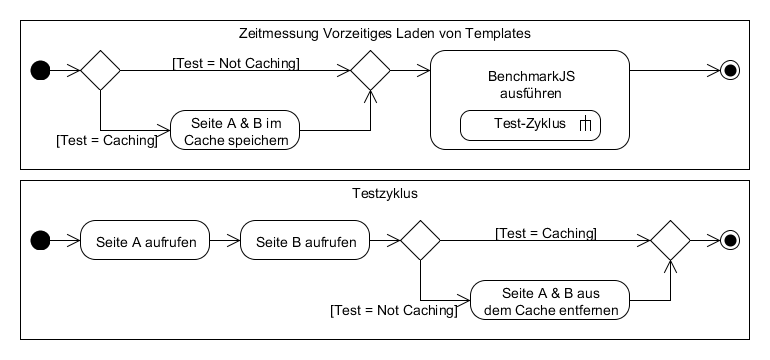
\includegraphics[scale=0.5]{Bilder/Testablauf-TemplatePrefetching.png}
	\caption{Testablauf für das Zwischenspeichern von Templates}
	\label{test-templateprefetching}
\end{figure}
In jedem Testzyklus wird zunächst die Seite des Untermoduls aufgerufen. AngularJS sendet nach durchgeführtem Seitenwechsel ein Event, woraufhin zurück zur vorherige Seite gewechselt wird. Dieser Vorgang wird durch die Algorithmen von BenchmarkJS mehrfach wiederholt. Vor dem gesamten Testvorgang wird beim Test mit Zwischenspeicherung dafür gesorgt, dass sich die Seiten im Zwischenspeicher befinden. Bei der Variante ohne Zwischenspeicherung wird der Zwischenspeicher nach jedem Testzyklus geleert. Getestet wird demnach das Wechseln zu und von einer Seite der Anwendung. Die Zeitmessung repräsentiert dadurch einen Test-Zyklus und gibt keine Auskunft über die erforderliche Zeit für einen konkreten Seitenwechsel. Relevant ist daher das Verhältnis beider Messungen. 
\begin{table}[h]
	\centering
\begin{tabular}{|l|l|l|}
	\hline
	\rowcolor[HTML]{C0C0C0} 
	\textbf{} & \textbf{Android 4.3} & \textbf{Android 4.4.4} \\ \hline
	ohne Caching & 182,607 & 273,105 \\ \hline
	Caching & 138,643 & 206,203 \\ \hline
	Steigerung & 24\% & 24\% \\ \hline
\end{tabular}
	\caption{Seitenübergänge, Vorzeitiges Laden von Templates, BenchmarkJS Laufzeitanalyse}
	\label{su-template-prefetching-benchjs-analyse}	
\end{table}
Das Ergebnis dieser Analyse ist in Tabelle \ref{su-template-prefetching-benchjs-analyse} aufgeführt. Durch diese Messung wird deutlich, dass das Zwischenspeichern eines Templates den Seitenaufruf im Schnitt um 24\% beschleunigt. Dieser Wert hängt direkt mit der Größe des \gls{html}-Templates zusammen. Denn je größer das Template ist, desto länger dauert das Abrufen über die Netzwerkschnittstelle. Für große Templates lohnt sich dieses Prinzip deshalb mehr als für kleine Templates. In diesem Beispiel wurde ein Template mit 84 \gls{dom}-Elementen und einer Größe von 8kb verwendet, was als Referenzwert dienen soll. 

\subsubsection{Lösungsansätze}
An dieser Stelle werden zwei Varianten betrachtet, mit denen ein vorzeitiges Laden von Templates implementiert werden kann. Beide Varianten erfordern Kenntnisse über den Aufbau und die kritischen Bereiche einer Anwendung. Die erste Variante benötigt einen geringen Implementierungsaufwand. Die als kritisch eingestuften Seiten werden dabei während dem Start der Anwendung geladen und zwischengespeichert. Als kritisch werden an dieser Stelle Seiten einer Anwendung bezeichnet, bei denen eine gute Performance essentiell ist. Abbildung \ref{su-tp-v1} zeigt diesen Vorgang für zwei Seiten einer Anwendung. Mittels der Methode \emph{run()} von AngularJS kann Logik beim Start der Anwendung ausgeführt werden. Mittels \emph{\$http} und \emph{\$templateCache} werden die Seiten anschließend abgerufen und zwischengespeichert. Bei einem Seitenwechsel zu einer Seite, die sich bereits im Zwischenspeicher befindet, wird nicht erst das Template geladen, sondern direkt aus dem Cache verwendet.  
\begin{lstlisting}[language=JavaScript, caption={Seitenübergänge, Vorzeitiges Laden von Templates Variante 1}\label{su-tp-v1}]
var app = angular.module('myApp');
app.run(function($http, $templateCache) {
	$http.get('/view1.html', { cache: $templateCache });
	$http.get('/view2.html', { cache: $templateCache });
});
\end{lstlisting}
Enthält die Anwendung viele kritische Seiten oder soll das vorzeitige Laden zur Verbesserung der Benutzerfreundlichkeit auf allen Seiten der Anwendung eingesetzt werden, ist diese Methode nicht praktikabel. Es müssten zu viele Seiten beim Start der Anwendung parallel geladen werden, was die Problematik aus Abschnitt \ref{pt-tp-main} und \ref{browser-engines} hervorruft.  
\\\\
Für die zweite Variante ist eine detaillierte Übersicht aller Seiten und ihrer Verknüpfungen untereinander erforderlich. Diese Verknüpfungen könnten über einen Zustandsgraphen visualisiert werden. Jede Seite bildet einen Knoten (Zustand) und Verknüpfungen zu anderen Seiten sind Kanten (Zustandsübergänge). Das Prinzip dieser Methodik besteht nun darin, alle Nachbarn einer Seite im Cache zu speichern, sobald sie selbst geladen wird. Bei vielen Verknüpfungen untereinander ist zusätzlich eine Gewichtung einzelner Verknüpfungen sinnvoll. Häufig frequentierte Seitenübergänge können dadurch priorisiert werden. Die Abbildung \ref{su-tp-v2} zeigt die Implementierung dieses Verfahrens. Neben der Routing-Konfiguration ist außerdem eine Datenstruktur für den Zustandsgraphen erforderlich. Nach Seitenübergängen sendet AngularJS das Event \emph{\$stateChangeSuccess}. Zu diesem Zeitpunkt werden alle Nachbarn einer Seite über den Zustandsgraphen ermittelt, anhand der Gewichtung sortiert und anschließend asynchron zwischengespeichert. Seiten, die bereits im Zwischenspeicher vorhanden sind, werden dabei ignoriert.
\begin{lstlisting}[language=JavaScript, caption={Seitenübergänge, Vorzeitiges Laden von Templates Variante 2}\label{su-tp-v2}]
function CompareWeight(a, b) {
	return b.weight - a.weight;
}

var nodes = [{ id: 'A', ... }, 
       { id: 'B', ... }, 
       { id: 'C', ... }
];

var relations = {
	'A': [ { id: 'B', weight: 0 } ],
	'B': [ { id: 'A', weight: 0 }, { id: 'C', weight: 1 } ],
	'C': [ { id: 'B', weight: 0 }, { id: 'A', weight: 1 } ],
};

nodes.forEach(function (r) {
	$stateProvider.state(r.id, r);
});

$rootScope.$on('$stateChangeSuccess', 
	function (event, toState, toParams, fromState, fromParams) {
	relations[toState.id]
		.sort(CompareWeight)
		.forEach(function (relation) {
			var node = nodes[relation.id];
			if ($templateCache.get(node.templateUrl)) return;
			$http.get(node.templateUrl, { cache: $templateCache } );
	});
});
\end{lstlisting}
Durch diese Methodik lässt sich vorzeitiges Laden für alle Seiten einer Anwendung realisieren, ohne die Performance bei einem Seitenwechsel zu beeinflussen. Zusätzlich ist dieses Verfahren unabhängig von der restlichen Implementierung, wodurch bei Änderungen an der Anwendung nur der Zustandsgraph aktualisiert werden muss. 